
\section{离散\trValuationRing{}与代数哈托格斯引理}

（余）维数 $1$ 的情形是重要的，因为如果你懂得了被维数 $1$ 隔开的诸\trPrimeIdeal{}如何行事，那么你就可以用归纳法证明任意维数下的事实。这正是\trKrull{}\trPrincipalIdealTheorem~12.3.3 如此有用的原因之一。

一个维数为 $1$ 的\trRegular\trLocalRing{}可以被看作「一条\trSmooth{}\trCurve{}的\trGerm」（见\cref{fig:germ-of-curve}）。心里可以记着两个例子：$k[x]_{(x)}=\{f(x)/g(x)\ :\ x\nmid g(x)\}$ 与 $\mathbb{Z}_{(5)}=\{a/b\ :\ 5\nmid b\}$。第一个例子是「几何的」，第二个例子是「算术的」，但希望显然的是：二者有某种根本的共同点。

\begin{figure}[htbp]
\centering
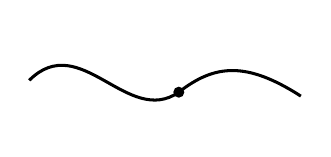
\begin{tikzpicture}[line width=1.1pt]
  \draw (-1.7,0.05) .. controls (-1.05,0.70) and (-0.45,-0.55) .. (0.20,-0.10) .. controls (0.65,0.25) and (1.05,0.30) .. (1.75,-0.15);
  \fill (0.20,-0.10) circle (0.07);
\end{tikzpicture}
\caption{一条\trCurve{}的\trGerm。（依原书手绘图重绘。）}\label{fig:germ-of-curve}
\end{figure}

本节的目的，是给出这些环的一长串彼此等价的定义。在开始之前，我们先把这七个定义迅速勾画一遍。一个\trNoetherian\trLocalRing{}可以「好」起来的方式有好几种。它可以是\trRegular{}的，可以是\trPID，可以是\trUFD，也可以是\trNormal{}的。在维数 $1$ 时，这些说法彼此相同。同样等价的是关于\trIdeal{}的几条好性质：$\mathfrak{m}$ 是\trPrincipalIdeal；或者\emph{所有}\trIdeal{}要么是\trMaximalIdeal{}的幂，要么是 $0$。最后，这个环可以带有一个离散\trValuation（discrete valuation）——一种对元素「大小」的度量，其表现格外良好。

\textbf{13.5.1.\ \trhTheorem{}。}\ ——\ \emph{设 $(A,\mathfrak{m})$ 是维数为 $1$ 的\trNoetherian\trLocalRing。则下列诸条彼此等价。}
\begin{enumerate}[label=(\alph*)]
\item \emph{$(A,\mathfrak{m})$ 是\trRegular{}的。}
\item \emph{$\mathfrak{m}$ 是\trPrincipalIdeal。}
\end{enumerate}

\emph{证明。}\ (a) 蕴涵 (b) 的理由如下。若 $A$ 正则，则 $\mathfrak{m}/\mathfrak{m}^2$ 是一维的。任取一个元素 $t\in\mathfrak{m}\setminus\mathfrak{m}^2$。那么 $t$ 生成 $\mathfrak{m}/\mathfrak{m}^2$，于是由\trNakayama{}引理~8.2.H，它生成 $\mathfrak{m}$（由\trNoetherian{}假设，$\mathfrak{m}$ 是有限生成的）。我们把这样的元素称为一个\textbf{\trUniformizer}（uniformizer）。

反过来，若 $\mathfrak{m}$ 在 $A$ 上由一个元素 $t$ 生成，则 $\mathfrak{m}/\mathfrak{m}^2$ 在 $A/\mathfrak{m}=k$ 上由一个元素 $t$ 生成。由定理~12.3.12，$\dim_k\mathfrak{m}/\mathfrak{m}^2\ge1$，于是 $\dim_k\mathfrak{m}/\mathfrak{m}^2=1$，所以 $(A,\mathfrak{m})$ 是正则的。\hfill$\square$

我们马上会用到一条有用的事实，它由几何动机驱动，并且是一条重要结果——\trArtin--\trRees（Artin--Rees）引理~13.9.3 的特例。我们将在 \S13.9 中证明它。

\textbf{13.5.2.\ \trhProposition{}。}\ ——\ \emph{若 $(A,\mathfrak{m})$ 是\trNoetherian\trLocalRing，则 $\bigcap_i\mathfrak{m}^i=0$。}

\textbf{13.5.3.}\quad 几何直观是：在一个点处「解析地为零」的函数（在各阶都消失）实际上在该点的一个开邻域内消失。（\mbox{练习~13.9.B}将把这件事说得更精确。）这个几何直观还提示了一个例子，表明\trNoetherian{}性是必要的：考虑 $\mathbb{R}$ 上原点处 $C^{\infty}$ 函数的芽环中的 $e^{-1/x^2}$。（特别地，这蕴涵：$\mathbb{R}$ 上 $C^{\infty}$ 函数的环在原点处的\trLocalization{}不是\trNoetherian{}的！）

人们忍不住想论证
\begin{equation*}\tag{13.5.3.1}\label{eq:m-powers-intersection}
\mathfrak{m}\bigl(\textstyle\bigcap_i\mathfrak{m}^i\bigr)=\textstyle\bigcap_i\mathfrak{m}^i,
\end{equation*}
然后用\trNakayama{}引理~8.2.9 论证 $\bigcap_i\mathfrak{m}^i=0$。遗憾的是，第一个等式是否为真并不显然：一般地，乘法与无穷递降交并不交换。（旁注：一般地，乘法与有限交也不交换，例如在 $k[x,y,z]/(xz-yz)$ 中，$(z)\bigl((x)\cap(y)\bigr)\neq(xz)\cap(yz)$。）我们将在\mbox{练习~13.9.A(b)} 中建立命题~13.5.2。（其实我们本可以现在就直接证明它，不太费事。）

\textbf{13.5.4.\ \trhTheorem{}。}\ ——\ \emph{设 $(A,\mathfrak{m})$ 是维数为 $1$ 的\trNoetherian\trLocalRing。则 (a) 与 (b) 等价于：}
\begin{enumerate}[label=(\alph*),start=3]
\item \emph{$A$ 是一个\trIntegralDomain，并且所有\trIdeal{}都具有形状 $\mathfrak{m}^n$（$n\ge0$）或 $(0)$。}
\end{enumerate}

\emph{证明。}\ 设 (a) 成立：设 $(A,\mathfrak{m},k)$ 是一个维数为 $1$ 的\trRegular\trLocalRing。我声称：对任何 $n$ 都有 $\mathfrak{m}^n\neq\mathfrak{m}^{n+1}$。否则，由\trNakayama{}引理，$\mathfrak{m}^n=0$，从而 $t^n=0$。但 $A$ 是\trIntegralDomain（由定理~13.2.11），于是 $t=0$，从而 $A=A/\mathfrak{m}$ 是一个域，而域的维数不是 $1$，矛盾。

我接着声称 $\mathfrak{m}^n/\mathfrak{m}^{n+1}$ 的维数为 $1$。理由：$\mathfrak{m}^n=(t^n)$。于是 $\mathfrak{m}^n$ 作为 $A$-模由一个元素生成，而 $\mathfrak{m}^n/(\mathfrak{m}\mathfrak{m}^n)$ 作为 $(A/\mathfrak{m}=k)$-模由一个元素生成（由上一段，它非零），所以它是一个一维\trVectorSpace。

于是我们有\trIdeal{}链 $A\supset\mathfrak{m}\supset\mathfrak{m}^2\supset\mathfrak{m}^3\supset\cdots$，满足 $\bigcap\mathfrak{m}^i=(0)$（命题~13.5.2）。我们想说：除这些之外，再没有别的\trIdeal{}的容身之处，因为每一对都被「维数 $1$」隔开，而且「末端没有余地」。证明：设 $I\subset A$ 是一个\trIdeal。若 $I\neq(0)$，则存在某个 $n$，使得 $I\subset\mathfrak{m}^n$ 但 $I\not\subset\mathfrak{m}^{n+1}$。取 $u\in I\setminus\mathfrak{m}^{n+1}$。那么 $(u)\subset I$。但 $u$ 生成 $\mathfrak{m}^n/\mathfrak{m}^{n+1}$，于是由\trNakayama{}引理它生成 $\mathfrak{m}^n$，所以我们得到 $\mathfrak{m}^n\subset I\subset\mathfrak{m}^n$，证毕：(c) 成立。

现在我们来证明 (c) 蕴涵 (a)。设 (a) 不成立：设我们有一个维数为 $1$ 的\trNoetherian{}局部\trIntegralDomain，它不正则，于是 $\mathfrak{m}/\mathfrak{m}^2$ 的维数至少为 $2$。任取 $u\in\mathfrak{m}-\mathfrak{m}^2$。那么 $(u,\mathfrak{m}^2)$ 是一个\trIdeal，但 $\mathfrak{m}^2\subsetneq(u,\mathfrak{m}^2)\subsetneq\mathfrak{m}$。\hfill$\square$

\textbf{13.5.A.（容易的练习）}\quad 设 $(A,\mathfrak{m})$ 是维数为 $1$ 的\trNoetherian\trLocalRing。证明：上面的 (a)--(c) 均等价于：
\begin{enumerate}[label=(\alph*),start=4]
\item \emph{$A$ 是一个\trPID。}
\end{enumerate}

\textbf{13.5.5.\ \trDVR。}\quad 我们接下来定义\trDVR{}的观念。设 $K$ 是一个域。$K$ 上的一个\textbf{离散\trValuation}（discrete valuation）是一个满同态 $v\colon K^{\times}\to\mathbb{Z}$（特别地，$v(xy)=v(x)+v(y)$），它满足
\[
v(x+y)\ge\min\bigl(v(x),v(y)\bigr)
\]
除非 $x+y=0$（此时左边无定义）。（这样的\trValuation{}称为\emph{\trNonArchimedean}的（non-Archimedean），尽管我们不会使用这个术语。）写下 $v(0)=\infty$ 往往是方便的。更一般地，一个\textbf{\trValuation}（valuation）是一个到全序\trAbelian{}群 $G$ 的满同态 $v\colon K^{\times}\to G$，尽管这对我们来说不那么重要。记号「val」将用来表示\trValuation。

这里有三个关键例子。
\begin{enumerate}[label=(\roman*)]
\item \emph{（$5$~进\trValuation）}$K=\mathbb{Q}$，$v(r)$ 是「出现在 $r$ 中的 $5$ 的幂」，例如 $v(35/2)=1$、$v(27/125)=-3$。
\item $K=k(x)$，$v(f)$ 是「出现在 $f$ 中的 $x$ 的幂」。
\item $K=k(x)$，$v(f)$ 是次数的相反数。这其实与 (ii) 是同一回事，只需把 $x$ 换成 $1/x$。
\end{enumerate}

于是 $\{0\}\cup\{x\in K^{\times}\ :\ v(x)\ge0\}$ 是一个环，我们把它记作 $\OO_v$。它称为 $v$ 的\textbf{\trValuationRing}（valuation ring）。（并非每个\trValuation{}都是离散的。考虑某个域 $k$ 上的\emph{\trPuiseux{}级数}（Puiseux series）环，$K=\bigcup_{n\ge1}k\bigl((x^{1/n})\bigr)$，\trValuation $v\colon K^{\times}\to\mathbb{Q}$ 由 $v(x^q)=q$ 给出。）

\textbf{13.5.B.（练习）}\quad 描述上面三个例子 (i)--(iii) 中的\trValuationRing。（你会注意到，它们是眼熟的维数为 $1$ 的\trNoetherian\trLocalRing。多么巧合！）

\textbf{13.5.C.（练习）}\quad 证明：$\{0\}\cup\{x\in K^{\times}\ :\ v(x)>0\}$ 是这个\trValuationRing{}的唯一\trMaximalIdeal。（提示：证明补集中的每个元素都可逆。）于是，\trValuationRing{}是一个局部环。

设 $A$ 是一个\trIntegralDomain。若存在其\trFractionField{} $K=K(A)$ 上的一个离散\trValuation $v$ 使得 $\OO_v=A$，则称 $A$ 是一个\textbf{\trDVR}（discrete valuation ring，简称 DVR）。类似地，若存在 $K$ 上的一个\trValuation $v$ 使得 $\OO_v=A$，则称 $A$ 是一个\textbf{\trValuationRing}。

现在，若 $A$ 是维数为 $1$ 的\trRegular\trLocalRing，而 $t$ 是一个\trUniformizer（作为\trIdeal{}生成 $\mathfrak{m}$ 的一个元素，或者等价地，作为 $k$-\trVectorSpace{}生成 $\mathfrak{m}/\mathfrak{m}^2$ 的一个元素），那么 $A$ 的任何非零元素 $r$ 都落在某个 $\mathfrak{m}^n\setminus\mathfrak{m}^{n+1}$ 中，于是 $r=t^nu$，其中 $u$ 可逆（因为 $t^n$ 生成 $\mathfrak{m}^n$——由\trNakayama{}引理——而 $r$ 也如此），所以 $K(A)=A_t=A[1/t]$。于是\emph{$K(A)^{\times}$ 的任何元素都可以唯一地写成 $ut^n$}，其中 $u$ 可逆，$n\in\mathbb{Z}$。这样我们就可以定义一个\trValuation $v$：$v(ut^n)=n$。

\textbf{13.5.D.（练习）}\quad 证明：$v$ 是一个离散\trValuation。

\textbf{13.5.E.（练习）}\quad 反过来，设 $(A,\mathfrak{m})$ 是一个\trDVR。证明：$(A,\mathfrak{m})$ 是维数为 $1$ 的\trRegular\trLocalRing。（提示：证明诸\trIdeal{}都形如 $(0)$ 或 $I_n=\{r\in A\ :\ v(r)\ge n\}$，而 $(0)$ 与 $I_1$ 是仅有的两个\trPrimeIdeal。于是我们便有\trNoetherian{}性，以及维数 $1$。证明：$I_1/I_2$ 由 $I_1-I_2$ 中任何一个元素的像生成。）

于是我们证明了：

\textbf{13.5.6.\ \trhTheorem{}。}\ ——\ \emph{\trIntegralDomain{} $A$ 是满足 (a)--(d) 的维数为 $1$ 的\trNoetherian\trLocalRing，当且仅当}
\begin{enumerate}[label=(\alph*),start=5]
\item \emph{$A$ 是一个\trDVR。}
\end{enumerate}

\textbf{13.5.F.（练习）}\quad 证明：一个\trDVR{}上只有一个离散\trValuation。

\textbf{13.5.7.}\ \emph{\trhDefinition{}。}\quad 于是，任何维数为 $1$ 的\trRegular\trLocalRing{}都自带其\trFractionField{}上的一个唯一\trValuation。若一个元素的\trValuation{}为 $n>0$，我们称该元素有一个 $n$ \textbf{阶\trZeros}（zero of order）。若\trValuation{}为 $-n<0$，我们称该元素有一个 $n$ \textbf{阶\trPole}（pole of order）。在处理完 (f) 与 (g) 之后，我们马上会回到这件事。

\textbf{13.5.8.\ \trhTheorem{}。}\ ——\ \emph{设 $(A,\mathfrak{m})$ 是维数为 $1$ 的\trNoetherian\trLocalRing。则 (a)--(e) 均等价于：}
\begin{enumerate}[label=(\alph*),start=6]
\item \emph{$A$ 是一个\trUFD，}
\item \emph{$A$ 是一个\trIntegralDomain，并且在（其\trFractionField{}中）整闭。}
\end{enumerate}

\emph{证明。}\ (a)--(e) 显然蕴涵 (f)，因为我们有下面这种「愚蠢的」唯一分解：$A$ 的每个非零元素都可以唯一地写成 $ut^n$，其中 $n\in\mathbb{Z}^{\ge0}$，$u$ 可逆。

(f) 蕴涵 (g)，因为\trUFD{}在其\trFractionField{}中是整闭的（\mbox{练习~5.4.F}）。

剩下要检验 (g) 蕴涵 (a)--(e)。我们将证明 (g) 蕴涵 (b)。

设 $(A,\mathfrak{m})$ 是维数为 $1$ 的\trNoetherian{}局部\trIntegralDomain，在其\trFractionField{} $K(A)$ 中整闭。任取非零的 $r\in\mathfrak{m}$。那么 $S=A/(r)$ 是一个维数为 $0$ 的\trNoetherian\trLocalRing——它唯一的素是 $\mathfrak{m}$ 的像，为避免混淆我们把它记作 $\mathfrak{n}$。于是 $\mathfrak{n}^N=0$，其中 $N$ 充分大（命题~12.1.9）。从而存在某个 $n$，使得 $\mathfrak{n}^n=0$ 而 $\mathfrak{n}^{n-1}\neq0$。

现在到了论证的关键之处。于是在 $A$ 中，$\mathfrak{m}^n\subset(r)$ 但 $\mathfrak{m}^{n-1}\not\subset(r)$。取 $s\in\mathfrak{m}^{n-1}-(r)$。考虑 $s/r\in K(A)$。由于 $s\notin(r)$，有 $s/r\notin A$，而 $A$ 是整闭的，所以 $s/r$ 不在 $A$ 上整。

现在（在 $K(A)$ 之内）$\frac{s}{r}\mathfrak{m}\not\subset\mathfrak{m}$（否则 $\frac{s}{r}\mathfrak{m}\subset\mathfrak{m}$ 将蕴涵 $\mathfrak{m}$ 是一个忠实 $A[\frac{s}{r}]$-模，与\mbox{练习~8.2.I}矛盾）。但 $s\mathfrak{m}\subset\mathfrak{m}^n\subset rA$，所以 $\frac{s}{r}\mathfrak{m}\subset A$。于是 $\frac{s}{r}\mathfrak{m}=A$，由此 $\mathfrak{m}=\frac{r}{s}A$，所以 $\mathfrak{m}$ 是\trPrincipalIdeal。\hfill$\square$

\textbf{13.5.9.}\ \emph{例：$\Spec\mathbb{Z}[i]$ 是正则的。}\quad 对于「$\Spec\mathbb{Z}[i]$ 为何正则」（\mbox{练习~13.3.N}），我们现在有了一个更简单的解释。首先，$\mathbb{Z}[i]$ 是\trUFD（\S5.4.5(o)），从而是\trNormal{}的（\S5.4.6）。它的维数为 $1$，于是由定理~13.5.8，它的闭点（即余维数 $1$ 的点）都正则。它的\trGenericPoint{}也正则，因为 $\mathbb{Z}[i]$ 是一个\trIntegralDomain。

\textbf{13.5.10.}\ \emph{例：「曲线几乎处处正则」。}\quad 由定理~13.5.8 与\mbox{练习~10.7.O}，每个一维\trVariety{}都除去有限多个\trClosedPoint{}外正则。

\textbf{13.5.11.}\ \emph{题外话：\trDedekindDomain。}\quad 一个\textbf{\trDedekindDomain}（Dedekind domain）是一个维数至多为 $1$ 的\trNoetherian\trIntegralDomain，它是\trNormal{}的（在其\trFractionField{}中整闭）。把一个\trDedekindDomain{}在除 $(0)$ 以外的任何一个素（即余维数 $1$ 的素）处取\trLocalization，得到的便是一个\trDVR。这是一个重要的概念，但我们不会多用它。数域的\trRingOfIntegers{}就是例子；见 \S10.7.1。特别地，若 $n$ 是一个模 $4$ 同余于 $3$ 的\trSquareFree{}整数，则 $\mathbb{Z}[\sqrt{n}]$ 是\trDedekindDomain（\mbox{练习~5.4.I(a)}）。如果你愿意，你可以证明\emph{\trDedekindDomain{}中\trIdeal{}的唯一分解}：非零理想都可以唯一地分解成\trPrimeIdeal。（提示：\trJordan--\trHolder{}的成套结果，\S6.5。）用与 \S13.5.9 中相同的论证，可知\trDedekindDomain{}都是正则的。

\textbf{13.5.12.\ \trNoetherian{}概形上函数的\trZeros{}与\trPole。}\quad 我们现在来推广下面这件事的说法：$\mathbb{A}^1_\mathbb{C}$ 上的 $(x-2)^2/(x-3)^4$ 在 $x=2$ 处有一个二阶\trZeros，在 $x=3$ 处有一个四阶极点。

\textbf{13.5.13.}\ \emph{\trhDefinition{}：余维数 $1$ 处正则（$\mathrm{R}_1$）。}\quad 我们称一个\trNoetherian{}环 $A$ 是\textbf{在余维数 $1$ 处正则}的（regular in codimension 1，简称 $\mathrm{R}_1$），若它在所有余维数 $1$ 的素处的\trLocalization{}都是\trRegular\trLocalRing。我们称一个\trLocally\trNoetherian{}概形 $X$ 是\textbf{在余维数 $1$ 处正则}的（regular in codimension 1，简称 $\mathrm{R}_1$），若它在它的余维数 $1$ 的点处正则。由定理~13.5.8，\trNoetherian{}正规概形都在余维数 $1$ 处正则。

\textbf{13.5.14.}\ \emph{\trhDefinition{}：在 $\mathrm{R}_1$ 点处的\trValuation。}\quad 设 $X$ 是一个\trLocally\trNoetherian{}概形\footnote{原书此处把该局部诺特概形记作（scheme $A$）（与同段环 $A$ 相撞），当系 $X$ 之误，径改。——译者注}。那么，对任何一个正则的余维数 $1$ 的点 $p$（即任何使 $\OO_{X,p}$ 成为维数为 $1$ 的\trRegular\trLocalRing{}的点 $p$），我们都有一个离散\trValuation $\mathit{val}_p$。若 $f$ 是 $\OO_{X,p}$ 的\trFractionField{}的任何一个非零元素（例如，若 $X$ 是整的，而 $f$ 是 $X$ 的\trFunctionField{}的一个非零元素），则当 $\mathit{val}_p(f)>0$ 时，我们称 $f$ \textbf{在 $p$ 处有} $\mathit{val}_p(f)$ \textbf{阶\trZeros}；而当 $\mathit{val}_p(f)<0$ 时，我们称 $f$ \textbf{在 $p$ 处有} $-\mathit{val}_p(f)$ \textbf{阶\trPole}。（我们尚不容许在一个并非正则的余维数 $1$ 点处讨论消失阶。定义倒是可以作出来，但它的表现可不如有离散\trValuation{}时那么好。\footnote{原书此处作（when have you have a discrete valuation），「have」当系衍词，径删。——译者注}）你能看出为什么 $75/34$ 在 $5$ 处有一个二阶\trZeros、在 $2$ 处有一个一阶极点吗？你能描述 $x^3(x+y)/(x^2+y)^3$ 在 $\mathbb{A}^2_k$ 上的\trZeros{}与极点吗？

\textbf{13.5.G.（练习：\trNoetherian{}概形上\trZeros{}与极点的有限性）}\quad 设 $X$ 是一个整的\trNoetherian{}概形，而 $f\in K(X)^{\times}$ 是其\trFunctionField{}的一个非零元素。证明：$f$ 只有有限多个\trZeros{}与极点。（提示：化归到 $X=\Spec A$。若 $f=f_1/f_2$，其中 $f_i\in A$，先对每个 $f_i$ 证明这条结果。）

\textbf{13.5.15.}\ \emph{\trhRemark{}。}\quad 一个（\trNoetherian{}）概形可以在余维数 $2$ 处\trSingular{}却依然\trNormal。例如，你已经证明过：在特征不为 $2$ 时，$\mathbb{A}^3$ 中的锥面 $x^2+y^2=z^2$ 是\trNormal{}的（\mbox{练习~5.4.I(b)}），但它在原点处\trSingular（\trZariski{}\trTangentSpace{}一眼望去就是三维的）。

但正规概形的奇性在某些方面并不算太糟：我们很快（\S13.5.18）就会为\trNoetherian{}正规概形讨论代数\trHartogs{}引理~13.5.19，它说的是：你可以把函数越过余维数 $2$ 的集合延拓出去。

\textbf{13.5.16.}\ \emph{\trhRemark{}。}\quad 我们知道，对\trNoetherian{}环有如下蕴含关系：
\[
\text{唯一分解整环}\;\Longrightarrow\;\text{整闭}\;\Longrightarrow\;\text{在余维数~1 处正则}
\]
于是，对\trLocally\trNoetherian{}概形，我们也有类似的蕴含关系：
\[
\text{唯一分解}\;\Longrightarrow\;\text{正规}\;\Longrightarrow\;\text{在余维数~1 处正则}
\]
这里有两个例子，向你表明这些包含关系都是严格的。

\textbf{13.5.H.（练习：\trPinchedPlane）}\quad 设 $A$ 是 $k[x,y]$ 的子环 $k[x^3,x^2,xy,y]$。（非正式地说：我们容许一切不含单项式 $x$ 的非零倍数的多项式。）证明：$\Spec k[x,y]\to\Spec A$ 是一个\trNormalization。证明：$A$ 不是整闭的。证明：$\Spec A$ 在余维数 $1$ 处正则。（最后一部分的提示：证明它是二维的，而当你把「原点」扔掉之后，得到的东西是正则的——办法是分别对 $x^2$ 与 $y$ 取逆，并考虑 $A_{x^2}$ 与 $A_y$。）

\textbf{13.5.17.}\ \emph{例（二次曲面再度登场）。}\quad 设 $k$ 是特征不为 $2$ 的\trAlgClosedField。那么 $k[w,x,y,z]/(wz-xy)$ 是整闭的，却不是\trUFD；见\mbox{练习~5.4.L}（以及\mbox{练习~13.1.E}）。

\textbf{13.5.18.\ \trNoetherian{}正规概形的代数\trHartogs{}引理。}\quad 多复变中的\trHartogs{}引理（非正式地）说：在一个余维数 $2$ 的集合之外定义的全纯函数，可以越过该集合延拓。我们现在来描述一个代数的类比，适用于\trNoetherian{}正规概形。（把它与黎曼第二延拓定理（Second Riemann Extension Theorem）作一番有益的比较也是可能的。）在 \S15.4 中把\trLineBundle{}与\trDivisor{}联系起来时，我们将反复地、不遗余力地使用这条结果。

\textbf{13.5.19.\ 代数\trHartogs{}引理。}\ ——\ \emph{设 $A$ 是一个整闭的\trNoetherian\trIntegralDomain。则}
\[
A=\bigcap\nolimits_{\mathfrak{p}\ \text{余维数 }1}A_{\mathfrak{p}}.
\]

这个等式在 $K(A)$ 之中成立；回忆：一个\trIntegralDomain{} $A$ 的任何\trLocalization{}都自然地是 $K(A)$ 的一个子集（\mbox{练习~1.2.C}）。警告：很少有人把这条引理称作代数\trHartogs{}引理。我这样称呼它，是因为它与复几何中的相应命题平行。

有人或许会这样说：若 $f\in K(A)$ 不落在 $A_{\mathfrak{p}}$ 中，其中 $\mathfrak{p}$ 的余维数为 $1$，则 $f$ 在 $[\mathfrak{p}]$ 处有一个极点；而若 $f\in K(A)$ 落在 $\mathfrak{p}A_{\mathfrak{p}}$ 中，其中 $\mathfrak{p}$ 的余维数为 $1$，则 $f$ 在 $[\mathfrak{p}]$ 处有一个\trZeros。

\textbf{13.5.20.}\quad 把代数\trHartogs{}引理在几何上解读为下述说法是值得的：\emph{\trNoetherian{}正规概形上没有极点的\trRationalFunction{}实际上是正则的（即它是 $A$ 的一个元素）。}非正式地说：「\trNoetherian{}正规概形具有\trHartogs{}性质。」

人们可以把代数\trHartogs{}引理更一般地陈述在 $\Spec A$ 是\trNoetherian{}正规概形的情形，意思是 $A$ 是若干个\trNoetherian{}正规\trIntegralDomain{}的乘积；读者不妨一试。

另一条推广（并且是某种更接近「正确」陈述的东西）是：若 $A$ 是域 $K$ 的一个子环，则 $A$ 在 $K$ 中的整闭包是 $K$ 的所有包含 $A$ 的\trValuationRing{}之交；说明与证明见 [AtM, Cor.~5.22]。

\textbf{13.5.21.}\ \hard\ \emph{代数\trHartogs{}引理~13.5.19 之证明。}\quad 证明中关键的妙招是下述构造。若 $A$ 是一个\trIntegralDomain，而 $r\in K(A)$，则 $r\in A$ 当且仅当对 $A$ 的所有\trPrimeIdeal{} $\mathfrak{p}$ 都有 $r\in A_{\mathfrak{p}}$，也就是说，$r$ 在 $\Spec A$ 的所有点处都正则。因此，问 $r\in K(A)$ 在哪些点处不正则是有意义的。我们的「分母理想」构造（来自命题~5.4.2\footnote{原书此处作（from the proof Proposition 5.4.2），当脱一「of」，径补。——译者注}的证明）表明这是一个闭子集：若 $I=\{a\in A\ :\ ar\in A\}$，则 $V(I)=\Supp A/I$ 的那些点 $[\mathfrak{p}]$ 恰好是 $r$ 不正则的点。我们从一个易于定义的模 $M^{a/b}$ 出发，可以对这个闭子集获得更精细的理解。

\textbf{13.5.22.}\quad 设 $r=a/b\notin A$，其中 $a,b\in A$。令 $\bar{a}$ 为 $a$ 在 $A/(b)$ 中的像。$r\notin A$ 这一事实意味着在 $A/(b)$ 中 $\bar{a}\neq0$。令 $M^{a/b}$ 为 $A/(b)$ 的由 $\bar{a}$ 生成的 $A$-子模。我们这样构造 $M^{a/b}$，使得 $M^{a/b}_q=0$ 当且仅当 $a/b\in A_q$\footnote{原书本节下标用斜体 $q$，而同段括注中又用 fraktur $\mathfrak{p}$（如 $A_{\mathfrak{p}}$），两种字形并存系原书自身不一致，兹照录。——译者注}。（翻译一下：$a$ 不是 $b$ 在 $A_{\mathfrak{p}}$ 中的倍数，当且仅当在 $A_{\mathfrak{p}}/(b)$ 中 $\bar{a}\neq0$。）

我们想证明代数\trHartogs{}引理，它说的是：若 $A$ 是整闭的，那么只需转而检验高度为 $1$ 的那些\trPrimeIdeal{}就够了。我们先给出这条事实的一个近似版本，它在没有「整闭」假设时也成立。

\textbf{13.5.23.\ \trhLemma{}。}\ ——\ \emph{设 $A$ 是一个\trNoetherian\trIntegralDomain，$r\in K(A)$。那么 $r\in A$ 当且仅当：对每个非零的 $g\in A$ 的每个\trPrimeIdeal{} $\mathfrak{p}\in\operatorname{Ass}(A/(g))$，都有 $r\in A_{\mathfrak{p}}$。}

\emph{证明。}\ 若 $r\in A$，则显然对一切 $\mathfrak{p}$ 都有 $r\in A_{\mathfrak{p}}$。故设 $r=a/b\notin A$。我们要找出一个这样的 $\mathfrak{p}$，使得 $r\notin A_{\mathfrak{p}}$，正如引理陈述中所描述的那样。我们取 $\mathfrak{p}$ 为 \S13.5.22 中构造的非零模 $M^{a/b}$ 的任一\trAssociatedPrimeIdeal。由于 $M^{a/b}$ 是 $A/(b)$ 的一个子模，$\mathfrak{p}$ 也是 $A/(b)$ 的\trAssociatedPrimeIdeal（\mbox{练习~6.6.G(a)}）。\hfill$\square$

\textbf{13.5.24.\ \trhProposition{}。}\ ——\ \emph{若 $A$ 是一个\trNoetherian{}整闭\trIntegralDomain，则}
\begin{enumerate}[label=(\roman*)]
\item \emph{$A$ 在余维数 $1$ 处正则（定义~13.5.13），}
\item \emph{对任何 $b\in A$，$A$-模 $A/(b)$ 没有\trEmbeddedPoint。}
\end{enumerate}

\emph{证明。}\ (i) 整闭性在\trLocalization{}下保持（\mbox{练习~5.4.A}），于是对每个余维数 $1$ 的素 $\mathfrak{p}$，$A_{\mathfrak{p}}$ 是整闭的。从而由定理~13.5.8，$A_{\mathfrak{p}}$ 正则。

(ii) 设 $\mathfrak{p}$ 是 $A/(b)$ 的一个\trAssociatedPrimeIdeal。我们想证明 $\mathfrak{p}$ 在 $A$ 中的余维数为 $1$。把 $A$ 换成其\trLocalization{} $A_{\mathfrak{p}}$，陈述的真值不变，所以只需证明下面这件事：「设 $(A,\mathfrak{m})$ 是一个\trNoetherian\trLocalRing，它是一个整闭\trIntegralDomain，且 $b\in\mathfrak{m}\setminus\{0\}$。设 $\mathfrak{m}\in\operatorname{Ass}(A/(b))$。那么 $\mathfrak{m}$ 是\trPrincipalIdeal（从而余维数至多为 $1$）。」

我们现在来证明这段话。取 $\bar{a}\in A/(b)$ 使得 $\operatorname{Ann}(\bar{a})=\mathfrak{m}$。那么 $\bar{a}\neq0$。把 $\bar{a}$ 提升为 $a\in A$。那么 $a/b\in K(A)\setminus A$，并且 $(a/b)\mathfrak{m}\subset A$。

我们用反证法证明 $(a/b)\mathfrak{m}\not\subset\mathfrak{m}$。假设不然。回忆\mbox{练习~8.2.I}：「设 $A$ 是 $K$ 的一个子环，$r\in K$，而 $N$ 是一个忠实 $A[r]$-模，它作为 $A$-模是有限生成的。那么 $r$ 在 $A$ 上整。」我们在这里以 $r=a/b$、$N=\mathfrak{m}$ 应用它。于是 $a/b$ 在 $A$ 上整，由 $A$ 的整闭性推出 $a/b\in A$，矛盾。

于是 $(a/b)\mathfrak{m}=A$，由此 $\mathfrak{m}=(b/a)A$，由此 $\mathfrak{m}$ 是\trPrincipalIdeal，正如所愿。\hfill$\square$

\textbf{13.5.25.\ \trhTheorem{}。}\ ——\ \emph{设 $A$ 是一个在余维数 $1$ 处正则的\trNoetherian\trIntegralDomain。则 (a) $A$ 是整闭的，当且仅当 (b) $A=\bigcap_{\mathfrak{p}\ \text{余维数 }1}A_{\mathfrak{p}}$。}

这条结果蕴涵代数\trHartogs{}引理~13.5.19。

\emph{证明。}\ (a) 蕴涵 (b)。我们应用引理~13.5.23。由命题~13.5.24(ii)，需要检验的素只剩下余维数 $1$ 的那些。

(b) 蕴涵 (a)。诸 $A_{\mathfrak{p}}$ 都是维数为 $1$ 的\trNoetherian{}整环且正则，从而由定理~13.5.8 是整闭的。设 $r\in K(A)$ 在 $A$ 上整。那么 $r\in K(A)$ 在每个余维数 $1$ 的 $\mathfrak{p}$ 处都对 $A_{\mathfrak{p}}$ 整，于是 $r\in A_{\mathfrak{p}}$，于是 $r\in\bigcap_{\mathfrak{p}\ \text{余维数 }1}A_{\mathfrak{p}}=A$。\hfill$\square$

我们以下面这条事实作结：日后（\S26.3）我们将把它与命题~13.5.24 一起，认作\trSerre{}的正规性 $\mathrm{R}_1+\mathrm{S}_2$ 判别法。

\textbf{13.5.26.\ \trhProposition{}。}\ ——\ \emph{设 $A$ 是一个满足命题~13.5.24 的条件 (i) 与 (ii) 的\trNoetherian\trIntegralDomain。那么 $A$ 是整闭的。}

\emph{证明。}\ 现在 $A=\bigcap_{\mathfrak{p}}A_{\mathfrak{p}}$，其中 $\mathfrak{p}$ 跑遍引理~13.5.23 所描述的那些素。由命题~13.5.24 的条件 (ii)，这些都是余维数 $1$ 的素。结论便由定理~13.5.25 结合命题~13.5.24 的条件 (i) 得出。\hfill$\square$

\textbf{13.5.27.}\ \emph{我们将会用到的代数\trHartogs{}引理~13.5.19 之推论。}

\textbf{13.5.I.（有用的练习）}\quad 设 $f$ 是一个\trLocally\trNoetherian{}正规概形上的非零\trRationalFunction。若 $f$ 没有极点，证明：$f$ 是正则的。
